\ifx\wholebook\relax \else
\documentclass[b5paper]{ctexart}
\usepackage[nomarginpar
  %, margin=.5in
]{geometry}

\addtolength{\oddsidemargin}{-0.05in}
\addtolength{\evensidemargin}{-0.05in}
\addtolength{\textwidth}{0.1in}
\usepackage[cn]{../../../prelude}

\setcounter{page}{1}

\begin{document}

\title{序列}

\author{刘新宇
\thanks{{\bfseries 刘新宇 } \newline
  Email: liuxinyu95@gmail.com \newline}
  }

\maketitle
\fi

\markboth{序列}{基本算法}

\ifx\wholebook\relax
\chapter{序列}
\numberwithin{Exercise}{chapter}
\fi

\section{简介}
\label{introduction}

序列是对数组和列表的一种抽象组合。我们希望理想的序列能达到下面的要求:

\begin{enumerate}
\item 可以在头部、尾部以常数时间插入、删除元素;
\item 可以快速(优于线性时间)连接两个序列;
\item 可以快速随机访问、更改任何元素;
\item 可以快速在指定位置断开序列。
\end{enumerate}

数组、列表仅部分满足这些要求,如下表所示。其中$n$为单个序列的长度,$n_1$、$n_2$分别表示被连接的两个序列的长度。

\btab{| l | c | r |}
  \hline
  操作 & 数组 & 列表 \\
  \hline
  在头部插入、删除 & $O(n)$ & $O(1)$ \\
  在尾部插入、删除 & $O(1)$ & $O(n)$ \\
  连接 & $O(n_2)$ & $O(n_1)$ \\
  随机访问 & $O(1)$ & 平均$O(n)$ \\
  在给定位置删除 & 平均$O(n)$ & $O(1)$ \\
  \hline
\etab

本章我们给出三种序列实现:二叉随机访问列表、可连接列表、手指树。

\section{二叉随机访问列表}
\index{序列!二叉随机访问列表}

二叉随机访问列表是由二叉树森林实现的随机访问列表。森林包含若干完全二叉树。元素只保存在叶子节点中。对任何非负整数$n$,将其表达为二进制,我们就知道需要多少棵完全二叉树来存储$n$个元素。每个值为1的二进制位代表一棵二叉树,树的大小对应着二进制位的高低。任给索引$1 \leq i \leq n$,我们都可以快速在森林中定位到保存第$i$个节点的二叉树。如图\ref{fig:bi-tree-sequence}所示,树$t_1$、$t_2$表示序列$[x_1, x_2, x_3, x_4, x_5, x_6]$。

\begin{figure}[htbp]
  \centering
  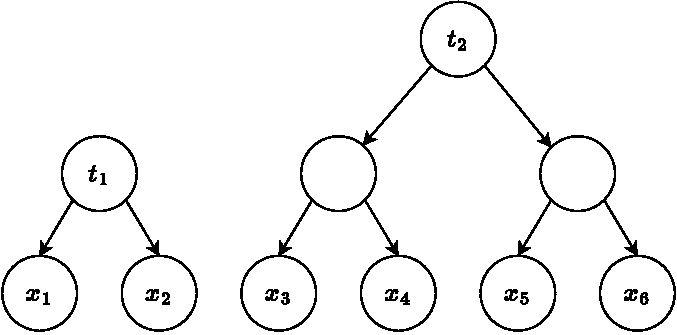
\includegraphics[scale=0.5]{img/bi-tree-sequence}
  \caption{含有6个元素的序列}
  \label{fig:bi-tree-sequence}
\end{figure}

记深度为$i+1$的完全二叉树为$t_i$。$t_0$只含有一个叶子节点。$t_i$含有$2^i$个叶子。对于$n$个元素的序列,我们把$n$表示为二进制数$n = (e_m e_{m-1} ... e_1 e_0)_2$,其中$e_i$为1或0。

\be
n = 2^0 e_0 + 2^1 e_1 + ... + 2^m e_m
\ee

如果$e_i \neq 0$,就需要一棵大小为$2^i$的完全二叉树$t_i$。在图\ref{fig:bi-tree-sequence}的例子中,序列长度为$6 = (110)_2$。最低位是0,我们不需要大小为1的树;第2位是1,需要一棵大小为2的树$t_1$;最高位是1,需要一棵大小为4的树$t_2$。这样就把序列$[x_1, x_2, ..., x_n]$表示为树的列表。列表中每棵树的大小都是唯一的,并按照从小到大排列。我们称之为\textbf{二叉随机访问列表}\cite{okasaki-book}。我们可以在二叉树定义的基础上稍作变化以实现这种列表:1、元素只保存在叶子节点中,2、在每棵子树中记录树的大小。这样每个分枝节点记为$(s, l, r)$,其中$s$表示子树的大小,$l$、$r$分别表示左右子树。包含元素$x$的叶子节点记为$(x)$。我们可以这样获取一棵树的大小:

\be
\begin{array}{rcl}
size\ (x) & = & 1 \\
size\ (s, l, r) & = & s \\
\end{array}
\ee

\index{二叉随机访问列表!插入}
为了把新元素$y$插入到序列$S$的前面,我们创建一棵只有一个叶子节点的$t_0$树:$t' = (y)$,然后把它插入到森林中。$insert\ y\ S = insert_T\ (y)\ S$,或写成克里化形式:

\be
insert\ y = insert_T\ (y)
\ee

我们检查森林中的第一棵树$t_i$,比较$t_i$和$t'$的大小,如果$t_i$较大,就将$t'$置于森林最前面(常数时间);若$t_i$和$t'$相等,我们将它们链接(常数时间)成一棵较大的树:$t'_{i+1} = (2s, t_i, t')$,然后递归地将$t'_{i+1}$插入到森林中。如图\ref{fig:bralist-2}所示。

\be
\begin{array}{rcl}
insert_T\ t\ [\ ] & = & [t] \\
insert_T\ t\ (t_1 \cons ts) & = & \begin{cases}
  size\ t < size\ t_1: & t : t_1 : ts \\
  \text{否则}: & insert_T\ (link\ t\ t_1)\ ts \\
  \end{cases}
\end{array}
\ee

其中$link$将两棵大小相同的树链接起来:$link\ t_1\ t_2 = (size\ t_1 + size\ t_2, t_1, t_2)$。

\begin{figure}[htbp]
  \centering
  \subcaptionbox{插入$x_1$。}{\hspace{0.2\textwidth}\includegraphics[scale=0.5]{img/bralst-1}\hspace{0.2\textwidth}}
  \subcaptionbox{插入$x_2$,链接产生$[t_1]$。}{\hspace{0.2\textwidth}\includegraphics[scale=0.5]{img/bralst-2}\hspace{0.2\textwidth}} \\
  \subcaptionbox{插入$x_3$,结果为$[t_0, t_1]$。}{\hspace{0.2\textwidth}\includegraphics[scale=0.5]{img/bralst-3}\hspace{0.2\textwidth}}
  \subcaptionbox{插入$x_4$。经两次链接后结果为$[t_2]$。}{\includegraphics[scale=0.5]{img/bralst-4}} \\
  \subcaptionbox{插入$x_5$,结果为:$[t_0, t_2]$。}{\includegraphics[scale=0.5]{img/bralst-5}}
  \subcaptionbox{插入$x_6$,结果为:$[t_1, t_2]$。}{\hspace{0.1\textwidth}\includegraphics[scale=0.5]{img/bralst-6}} \\
  \caption{插入$x_1, x_2, ..., x_6$}
  \label{fig:bralist-2}
\end{figure}

若森林中包含$m$棵树,$m$的大小为$O(\lg n)$,头部插入的性能为$O(\lg n)$。稍后我们证明分摊性能为$O(1)$。

\index{二叉随机访问列表!从头部删除}
对称地,我们利用插入的逆过程实现从序列头部删除元素。如果森林中第一棵树是$t_0$(单叶子节点),我们直接将$t_0$删除;否则,递归地将第一棵树拆分直到获得$t_0$,然后将其删除。如图\ref{fig:bralist-pop}所示。

\begin{figure}[htbp]
  \centering
  \subcaptionbox{序列$x_1, x_2, ..., x_5$对应森林$[t_0, t_2]$}{\includegraphics[scale=0.5]{img/bralst-5}}
  \subcaptionbox{删除$x_5$。直接删除$t_0$。}{\includegraphics[scale=0.5]{img/bralst-4}} \\
  \subcaptionbox{删除$x_4$。经过两次拆分后得到$[t_0, t_0, t_1]$,删除后得$[t_0, t_1]$。}{\hspace{0.2\textwidth}\includegraphics[scale=0.5]{img/bralst-3}\hspace{0.2\textwidth}}
  \caption{从头部删除元素}
  \label{fig:bralist-pop}
\end{figure}

\be
\begin{array}{rcl}
extract\ ((x) \cons ts) & = & (x, ts) \\
extract\ ((s, t_1, t_2) \cons ts) & = & extract\ (t_1 \cons t_2 \cons ts) \\
\end{array}
\ee

利用$extract$即可实现对头部元素的删除:

\be
\begin{cases}
head & = \textit{fst} \circ extract \\
tail & = \textit{snd} \circ extract \\
\end{cases}
\ee

其中$\textit{fst}\ (a, b) = a$, $\textit{snd}\ (a, b) = b$分别返回一对值中的两个部分。

\index{二叉随机访问列表!随机访问}
森林中的树实际上将元素划分为大小不同的区块。给定任意索引$1 \leq i \leq n$,我们先定位到对应的完全二叉树,然后再进行一次树查找就可定位到元素。

\begin{enumerate}
\item 比较$i$和森林中第一棵树$t$的大小,若$i \leq size(t)$,则元素在$t$中,接下来在树$t$中进行查找;
\item 否则,令$i' = i - size(t)$,然后递归地在剩余的树中查找第$i'$个元素。
\end{enumerate}

\be
(t \cons ts)[i] = \begin{cases}
  i \leq size\ t: & lookup_T\ i\ t \\
  \text{否则}: & ts[i - size\ t] \\
\end{cases}
\ee

其中$lookup_T$在树中进行二分查找。如果$i = 1$,我们返回根节点;否则,我们将树拆半,然后递归查找:

\be
\begin{array}{rcl}
lookup_T\ 1\ (x) & = & x \\
lookup_T\ i\ (s, t_1, t_2) & = & \begin{cases}
  i \leq \lfloor \dfrac{s}{2} \rfloor: & lookup_T\ i\ t_1 \\
  \text{否则}: & lookup_T\ (i - \lfloor \dfrac{s}{2} \rfloor)\ t_2 \\
  \end{cases}
\end{array}
\ee

图\ref{fig:get-at-example}描述了在一个长度为6的序列中查找第4个元素的步骤。第一棵树大小为2 < 4,继续检查第二棵树,并将索引更新为$i' = 4 - 2 $。接下来的树大小为$4 > i' = 2$,故待查找元素就在这棵树中。因为索引为2,不大于拆半的子树大小$4/2 = 2$,所以接下来检查左子树,然后检查右侧的孙子分支,最终得到要访问的元素。类似地,我们也可以修改任意位置$i$的元素。

\begin{figure}[htbp]
  \centering
  \subcaptionbox{$S[4], 4 > size(t_1) = 2$}{\includegraphics[scale=0.5]{img/bralst-6}}
  \subcaptionbox{$S'[4-2] \Rightarrow lookup_T\ 2\ t_2$}{\hspace{0.2\textwidth}\includegraphics[scale=0.5]{img/bralst-4}\hspace{0.2\textwidth}} \\
  \subcaptionbox{$ 2 \leq \lfloor \dfrac{size(t_2)}{2} \rfloor \Rightarrow lookup_T\ 2\ left(t_2)$}{\hspace{0.2\textwidth}\includegraphics[scale=0.5]{img/bralst-4l}\hspace{0.2\textwidth}}
  \subcaptionbox{$lookup_T\ 1\ right(left(t_2))$, 返回$x_3$}{\hspace{0.2\textwidth}\includegraphics[scale=0.5]{img/bralst-4lr}\hspace{0.2\textwidth}}
  \caption{获取$S[4]$}
  \label{fig:get-at-example}
\end{figure}

根据完全二叉树的性质,对于含有$n$个元素的序列,树木的棵数为$O(\lg n)$。对于索引$i$,最多需要$O(\lg n)$时间来定位到树。接下来的搜索和树的高度成正比,最多也是$O(\lg n)$。因此随机访问的总体性能为$O(\lg n)$。

\begin{Exercise}
如何处理索引越界情况?
\end{Exercise}

\section{数字表示}
\index{序列!二叉随机访问列表的数字表示}

非负整数$n$的二进制形式和森林之间存在关系:$n = 2^0e_0 + 2^1e_1 + ... + 2^me_m$,其中$e_i$为第$i$位的值。若$e_i = 1$,则存在一棵大小为$2^i$的完全二叉树。向序列头部插入元素,对应于二进制数加1;而删除对应二进制数减1。我们称这种关系为\underline{数字表示}\cite{okasaki-book}。为了明确表示这种对应,我们为每个二进制位定义两个状态:状态零$Zero$表示不存在二叉树,而状态一$One\ t$表示存在二叉树$t$。这样森林就可以表示为一组二进制状态的列表,从而把插入实现为二进制数的增加。

\be
\begin{array}{rcl}
add\ t\ [\ ] & = & [One\ t] \\
add\ t\ (Zero \cons ds) & = & (One\ t) : ds \\
add\ t\ (One\ t' \cons ds) & = & Zero : add\ (link\ t\ t')\ ds
\end{array}
\ee

将树$t$插入森林对应二进制加法:若森林为空,我们创建状态$One\ t$,它是二进制数中的唯一位。相当于$0 + 1 = 1$。若森林不空,如果二进制首位数字是$Zero$,我们创建一个状态$One\ t$替换掉$Zero$。这相当于二进制加法$(...digits...0)_2 + 1 = (...digits...1)_2$。例如$6 + 1 = (110)_2 + 1 = (111)_2 = 7$。如果二进制首位是$One\ t'$,我们认为$t$和$t'$的大小相同。这是因为我们总是以一个叶子$t_0 = (x)$开始插入,待插入树的大小逐渐增长,呈一个序列$1, 2, 4, ..., 2^i, ...$。我们将$t$和$t'$链接起来,递归地插入到剩余的数字中。而之前的$One\ t'$被替换为$Zero$。这相当于二进制加法$(...digits...1)_2 + 1 = (...digits'...0)_2$。例如$7 + 1 = (111)_2 + 1 = (1000)_2 = 8$。

接下来我们用二进制减法来表示删除。如果序列只含有一位$One\ t$,删除后序列变为空。这对应二进制减法$1 - 1 = 0$。如果序列有多位,并且首位是$One\ t$,我们将其替换为$Zero$。这相当于二进制减法 $(...digits...1)_2 - 1 = (...digits...0)_2$。例如$7 - 1 = (111)_2 - 1 = (110)_2 = 6$。如果首位是$Zero$,减法需要借位。我们递归地从剩余的数字中抽取树,将其分拆成两棵树$t_1$、$t_2$,将$Zero$替换成$One\ t_2$,并删除$t_1$。这相当于二进制减法$(...digits...0)_2 - 1 = (...digits'...1)_2$。例如$4 - 1 = (100)_2 - 1 = (11)_2 = 3$。

\be
\begin{array}{rcl}
minus\ [One\ t] & = & (t, [\ ]) \\
minus\ ((One\ t) \cons ts) & = & (t, Zero \cons ts) \\
minus\ (Zero \cons ts) & = & (t_1, (One\ t_2) \cons ts'), \text{其中}: (s, t_1, t_2) = minus\ ts \\
\end{array}
\ee

数字表示并没有改变复杂度。我们使用聚合方法法,分析在插入的分摊复杂度。考虑依次向空序列插入$n = 2^m$个元素的过程。森林的二进制表示如表\ref{tab:ralist-insertion}:

\begin{table}[htbp]
\centering
\begin{tabular}{|l|r|}
  \hline
  i & 二进制(高 ... 低) \\
  \hline
  0 & 0, 0, ..., 0, 0 \\
  1 & 0, 0, ..., 0, 1 \\
  2 & 0, 0, ..., 1, 0 \\
  3 & 0, 0, ..., 1, 1 \\
  ... & ... \\
  $2^m-1$ & 1, 1, ..., 1, 1 \\
  $2^m$ & 1, 0, 0, ..., 0, 0 \\
  \hline
  位变化次数 & 1, 1, 2, ... $2^{m-1}$, $2^m$ \\
  \hline
\end{tabular}
\caption{插入$2^m$个元素的过程}
\label{tab:ralist-insertion}
\end{table}

二进制表示的最低位每次插入时都变化,总共需要$2^m$次计算;次低位每隔一次变化,执行一次树的链接操作。共需要$2^{m-1}$次计算;次高位总共只变化一次,将所有的树链接成一棵大树。最后一个元素插入后,最高位变为1。将所有计算次数相加,得到$T = 1 + 1 + 2 + 4 + ... + 2^{m-1} + 2^m = 2^{m+1}$。平均每次插入操作的分摊复杂度为:

\be
O(T/n) = O(\frac{2^{m+1}}{2^m}) = O(1)
\ee

这就证明了插入的分摊复杂度为常数时间。

\begin{Exercise}
\Question{实现数值表示序列的随机访问$S[i], 1 \leq i \leq n$。其中$n$是序列长度。}
\Question{使用聚合法,证明删除的分摊复杂度为常数时间。}
\Question{可以用长度为$2^m$的数组表示完全二叉树($m$是非负整数)。请用数组实现二叉树森林的插入和随机访问。并分析它们的分摊复杂度。}
\end{Exercise}

\section{双数组序列}
\index{序列!双数组序列} \index{双数组列表!插入和添加}

在上一章中,我们给出过双数组队列。由于数组可以常数时间随机访问,我们可以将其扩展为双数组序列。如图\ref{fig:parrays},按头对头的方式连接两个数组。在列表的头部插入时,添加到$f$数组末尾;向尾部插入时,添加到$r$数组末尾。这样我们用一对数组表示列表$S = (f, r)$,令$\textproc{Front}(S) = f$,$\textproc{Rear}(S) = r$。插入、删除实现如下:

\begin{figure}[htbp]
  \centering
  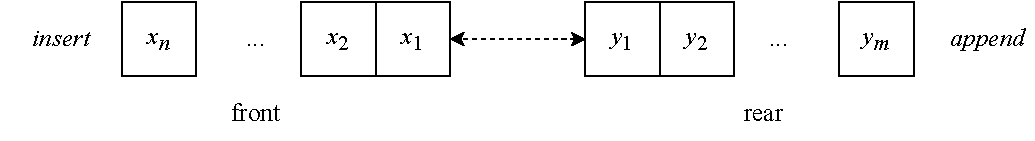
\includegraphics[scale=0.7]{img/parrays}
  \caption{双数组序列}
  \label{fig:parrays}
\end{figure}

\begin{algorithmic}[1]
\Function{Insert}{$x, S$}
  \State \textproc{Append}($x$, \Call{Front}{$S$})
\EndFunction
%\Statex
\Function{Append}{$x, S$}
  \State \textproc{Append}($x$, \Call{Rear}{$S$})
\EndFunction
\end{algorithmic}

\index{双数组列表!随机访问}
随机访问第$i$个元素时,我们先判断$i$索引到$f$还是$r$,然后再定位到元素。若$ i \leq |f|$,元素在$f$中。由于$f$和$r$头对头连接的,所以$f$按照从右向左逆序索引元素。我们用$|f| - i + 1$定位到元素;如果$i > |f|$,元素在$r$中。元素是从左向右索引的,我们用$i - |f|$定位到元素。

\begin{algorithmic}[1]
\Function{Get}{$i, S$}
  \State $f, r \gets $ \Call{Front}{$S$}, \Call{Rear}{$S$}
  \State $n \gets $ \Call{Size}{$f$}
  \If{$i \leq n $}
    \State \Return $f[n - i + 1]$ \Comment{反向索引}
  \Else
    \State \Return $r[i - n]$
  \EndIf
\EndFunction
\end{algorithmic}

\index{双数组列表!删除和平衡}
删除可能把一个数组$f$或$r$变空,而另一个仍有元素,需要恢复平衡。当$f$或$r$等于$[\ ]$时,我们将另一数组分成两半,然后将前一半反转形成一对新的数组。$f$、$r$是对称的。我们也可以交换$f$、$r$,递归调用\textproc{Balance},再把$f$、$r$交换回来。

\begin{algorithmic}[1]
\Function{Balance}{$S$}
  \State $f \gets$ \Call{Front}{$S$}, $r \gets$ \Call{Rear}{$S$}
  \State $n \gets$ \Call{Size}{$f$}, $m \gets$ \Call{Size}{$r$}
  \If{$F = [\ ]$}
    \State $k \gets \lfloor \dfrac{m}{2} \rfloor$
    \State \Return $(\textproc{Reverse}(r[1 ... k]), r[(k + 1) ... m])$
  \EndIf
  \If{$R = [\ ]$}
    \State $k \gets \lfloor \dfrac{n}{2} \rfloor$
    \State \Return $(f[(k + 1) ... n], \textproc{Reverse}(f[1 ... k]))$
  \EndIf
  \State \Return $(f, r)$
\EndFunction
\end{algorithmic}

在每次删除时,我们都检查$f$、$r$是否为空,并触发平衡操作:

\begin{algorithmic}[1]
\Function{Remove-Head}{$S$}
  \State \Call{Balance}{$S$}
  \State $f, r \gets$ \Call{Front}{$S$}, \Call{Rear}{$S$}
  \If{$f = [\ ]$} \Comment{$S = ([], [x])$}
    \State $r \gets [\ ]$
  \Else
    \State \Call{Remove-Last}{$f$}
  \EndIf
\EndFunction
\Statex
\Function{Remove-Tail}{$S$}
  \State \Call{Balance}{$S$}
  \State $f, r \gets$ \Call{Front}{$S$}, \Call{Rear}{$S$}
  \If{$r = [\ ]$} \Comment{$S = ([x], [])$}
    \State $f \gets [\ ]$
  \Else
    \State \Call{Remove-Last}{$r$}
  \EndIf
\EndFunction
\end{algorithmic}

由于要进行反转,双数组序列在最坏情况下性能为$O(n)$,其中$n$是元素个数。但是分摊复杂度是常数时间的。

\begin{Exercise}
\Question{证明双数组序列删除的分摊复杂度为常数时间。}
\end{Exercise}

\section{可连接列表}
\index{序列!可链接列表}

虽然我们可以用$O(\lg n)$时间在二叉树随机访问森林的头部进行插入、删除、索引,但连接两个序列并不容易。我们不能简单地将所有二叉树合并到一起,而需要不断链接大小相同的树。图\ref{fig:clist}给出了一种可连接列表的实现。多叉树的根存储序列的第一个元素$x_1$, 其它元素被分成若干片段保存在更小的序列中,每个片段是一棵子树。这些子树由一个实时队列(见上一章)管理,表示为$(x_1, Q_x) = [x_1, x_2, ..., x_n]$。当需要连接另一个列表$(y_1, Q_y) = [y_1, y_2, ..., y_m]$时,我们将其入队到$Q_x$的尾部。连接运算定义如下。实时队列的入队性能为常数时间,因此列表连接的性能也是常数时间的。

\begin{figure}[htbp]
  \centering
  \subcaptionbox{$(x_1, Q_x) = [x_1, x_2, ..., x_n]$}{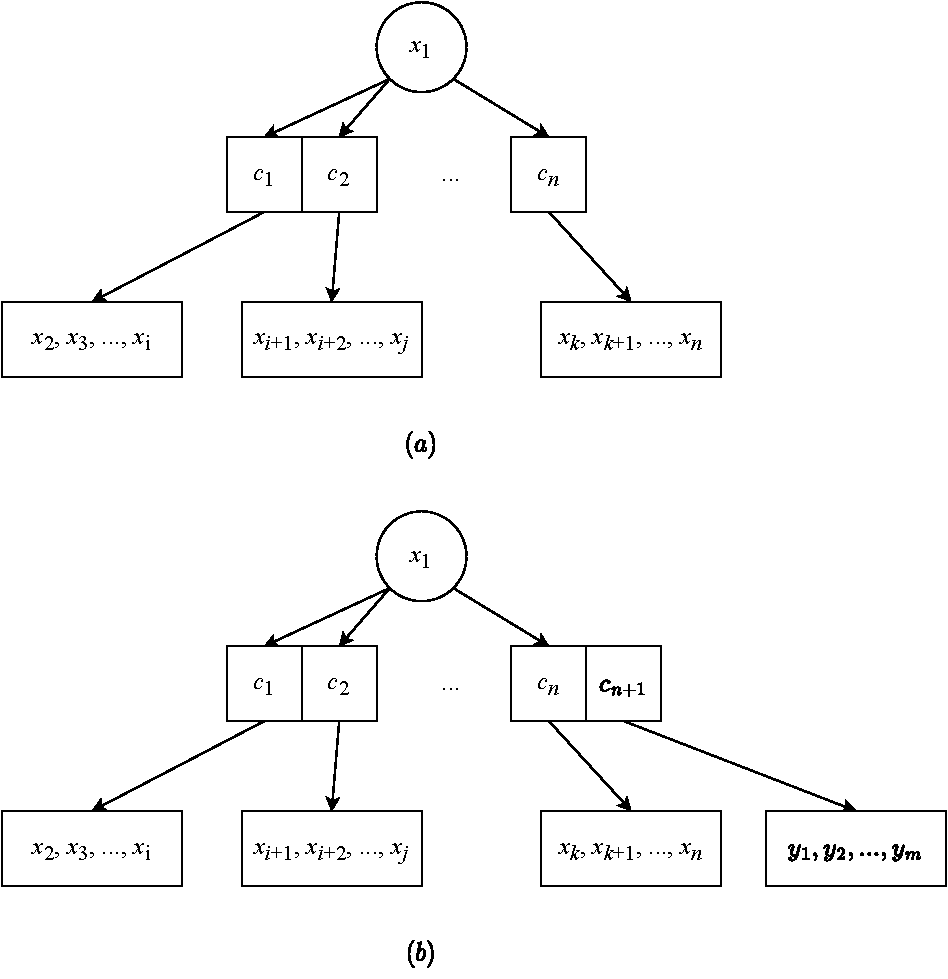
\includegraphics[scale=0.5]{img/clist}} \\
  \subcaptionbox{连接$(y_1, Q_y) = [y_1, y_2, ..., y_m]$相当于入队$c_{n+1}$到$Q_x$}{\includegraphics[scale=0.4]{img/clist1}}
  \caption{可连接列表}
  \label{fig:clist}
\end{figure}

\be
\begin{array}{rcl}
s \doubleplus \nil & = & s \\
\nil \doubleplus s & = & s \\
(x, Q) \doubleplus s & = & (x,\ push\ s\ Q) \\
\end{array}
\ee

插入新元素$z$时,我们先创建一个单元素列表$(z, \nil)$,然后将其连接起来。

\be
\begin{cases}
insert\ x\ s & = (x, \nil) \doubleplus s \\
append\ x\ s & = s \doubleplus (x, \nil) \\
\end{cases}
\ee

从可连接列表的头部删除元素需要单独的设计。$x_1$为根节点,删除后剩下的所有子树也都是由多叉树表示的可连接列表。我们可以把它们全部连接到一起,形成一个新列表。

\be
\begin{array}{rcl}
concat\ \nil & = & \nil \\
concat\ Q & = & (top\ Q) \doubleplus concat\ (pop\ Q) \\
\end{array}
\ee

全部子树存储在实时队列中。我们将第一棵子树$c_1$出队,然后递归地将剩余的子树连接在一起成为$s$,最后把$c_1$、$s$连接起来。我们使用$concat$从头部删除元素。

\be
tail\ (x, Q) = concat\ Q
\ee

算法$concat$遍历了队列,逐步归并到一个最终的结果。这本质上相当于对$Q$进行叠加操作\cite{learn-haskell}。

\be
\begin{array}{rcl}
fold\ f\ z\ \nil & = & z \\
fold\ f\ z\ Q & = & f\ (top\ Q)\ (fold\ f\ z\ (pop\ Q)) \\
\end{array}
\ee

其中$f$是用于归并的二元函数,$z$是零元。下面是一些队列叠加的例子,令$Q = [1, 2, ..., 5]$。

\[
\begin{array}{rcl}
fold\ (+)\ 0\ Q & = & 1 + (2 + (3 + (4 + (5 + 0)))) = 15 \\
fold\ (\times)\ 1\ Q\ & = & 1 \times (2 \times (3 \times (4 \times (5 \times 1)))) = 120 \\
fold\ (\times)\ 0\ Q & = & 1 \times (2 \times (3 \times (4 \times (5 \times 0)))) = 0 \\
\end{array}
\]

我们可以利用叠加来定义$concat$(克里化形式):

\be
concat = fold\ (\doubleplus)\ \nil
\ee

删除操作的性能在最坏情况下是线性的。当连续向空序列添加$n$个元素后,立即执行一次删除。此时多叉树中的$n-1$棵子树都是单元素的(只含有一个叶子节点)。$concat$需要$O(n)$时间进行归并。如果插入、添加、删除、连接随机发生,则分摊复杂度是常数时间的。

\begin{Exercise}
\Question{证明可连接列表的删除操作的分摊复杂度为常数时间的。} %Banker方法
\end{Exercise}

\section{手指树}
\index{序列!手指树}

二叉随机访问列表可以在头部用常数时间(分摊)插入、删除,以对数时间进行随机访问。但是难以向尾部添加元素、也无法进行快速连接。可连接列表能够用常数时间(分摊)进行连接,在头、尾部用常数时间插入。但不能用索引进行随机访问。这两个例子提示我们:1、需要某种方式快速访问头、尾以进行增删;带有递归的结构(例如树)可将随机访问转换成分而治之的搜索。手指树\cite{finger-tree-1977}利用了这两点来实现序列\cite{finger-tree-2006}。树是否平衡对搜索性能至关重要。手指树利用了2-3树(一种特殊的B-树)。一棵2-3树包含二或三棵子树,如:$(t_1, t_2)$或$(t_1, t_2, t_3)$。

\lstset{frame = single}
\begin{Haskell}
data Node a = Br2 a a | Br3 a a a
\end{Haskell}

最左侧的非叶子节点叫做$f$手指(或左侧手指),最右侧的非叶子节点叫做$r$手指(或右侧手指)\footnote{分别是英文前(front)、后(rear)的首字母。}。两个手指都是2-3树,并且所有的子节点都是叶子,它们实现为含有2到3个叶子的列表。当然手指树也可以为空或者含有单元素的叶子。归纳起来,我们定义一棵手指树为:

\begin{enumerate}
\item 或者为空$\nil$;
\item 或者是单元素叶子$(x)$;
\item 或者包含三部分:一棵子树和左、右手指,记为$(f, t, r)$。每个手指是一个至多3个元素的列表;
\end{enumerate}

\begin{Haskell}
data Tree a = Empty
            | Lf a
            | Tr [a] (Tree (Node a)) [a]
\end{Haskell}

\subsection{插入}

\begin{figure}[htbp]
  \centering
  \subcaptionbox{$\nil$}{\hspace{0.2\textwidth}\includegraphics[scale=0.5]{img/ftr-empty}\hspace{0.2\textwidth}}
  \subcaptionbox{$(x)$}{\hspace{0.2\textwidth}\includegraphics[scale=0.5]{img/ftr-leaf}\hspace{0.2\textwidth}} \\
  \subcaptionbox{$([b], \nil, [a])$}{\includegraphics[scale=0.5]{img/ftr-ab}}
  \caption{手指树,例1}
  \label{fig:ftr-example-1}
\end{figure}

\begin{figure}[htbp]
  \centering
  \subcaptionbox{向$f$手指插入3个元素后,超过了2-3树的限制,不再平衡。}{\includegraphics[scale=0.5]{img/ftr-abcde}}
  \hspace{0.2\textwidth}
  \subcaptionbox{恢复平衡。$f$手指含有2个元素;中间部分为叶子,包含一棵2-3树。}{\includegraphics[scale=0.5]{img/ftr-abcdef}}
  \caption{手指树,例2}
\label{fig:ftr-example-2}
\end{figure}

如图\ref{fig:ftr-example-1}和\ref{fig:ftr-example-2}所示。例1中(a)为$\nil$,(b)是插入一个元素后的结果。(c)含有两个元素,分别在$f$、$r$手指中。如果继续插入元素,$f$手指会超过2-3树的限制,如例2(a)所示。(b)恢复平衡后,$f$手指中有2个元素,中间部分是一个含有一棵2-3树的叶子。这些例子可以表示为:

\[
\begin{array}{ll}
\nil & \texttt{Empty}\\
(a) & \texttt{Lf a}\\
([b], \nil, [a]) & \texttt{Tr [b] Empty [a]}\\
([e, d, c, b], \nil, [a]) & \texttt{Tr [e, d, c, b] Empty [a]}\\
([f, e], (d, c, b), [a]) & \texttt{Tr [f, e] Lf (Br3 d c b) [a]}\\
\end{array}
\]

\index{手指树!头部插入}
注意最后一个例子中,中间部分的子树是一个叶子。手指树是递归的。除去$f$、$r$手指的中间部分是一棵更深的手指树,定义为$Tree\ (Node\ a)$。深度增加一级,就多嵌套一级。上面的例子实际描述了向手指树插入元素的过程。我们可以归纳如下。向一棵手指树$T$中插入$a$时:

\begin{enumerate}
\item 如果$T = \nil$,则结果为单元素叶子$(a)$;
\item 如果$T = (b)$是一个叶子,结果为$([a], \nil, [b])$;
\item $T = (f, t, r)$,如果$f$中元素个数不超过3,将$x$插入到$f$中,如果$f$中元素个数超过3。将$f$中的后3个元素移入一棵新的2-3树$t'$,递归地将$t'$插入到$t$中。最后将$x$插入到$f$中。
\end{enumerate}

\be
\begin{array}{rcl}
insert\ a\ \nil & = & (x) \\
insert\ a\ (b) & = & ([a], \nil, [b]) \\
insert\ a\ ([b, c, d, e], t, r) & = & ([a, b], insert\ (c, d, e)\ t, r) \\
insert\ a\ (f, t, r) & = & (a \cons f, t, r) \\
\end{array}
\ee

出了递归插入外,其它情况插入都需要常数时间。递归深度取决于树的高度$h$,由于使用2-3树并维持平衡,因此$h= O(\lg n)$,其中$n$是手指树中存储元素的个数。递归可以分摊到其它情况中,插入的分摊复杂度为常数时间\cite{okasaki-book}\cite{finger-tree-2006}。

\begin{Exercise}
\Question{消除递归,用循环的方式实现手指树插入。}
\end{Exercise}

\begin{Answer}
\Question{消除递归,用循环的方式实现手指树插入。
对于手指树$T = (f, t, r)$,令$\textproc{Mid}(T) = t$以获取中间部分。

\begin{algorithmic}[1]
\Function{Insert}{$x, T$}
  \State $n = (x)$
  \State $\perp \gets p \gets ([\ ], T, [\ ])$
  \While{$|\textproc{Front}(T)| \geq 3$}
    \State $f \gets \textproc{Front}(T)$
    \State $n \gets (f[2], f[3], ...)$
    \State $\textproc{Front}(T) \gets [n, f[1]]$
    \State $p \gets T$
    \State $T \gets$ \Call{Mid}{$T$}
  \EndWhile
  \If{$T =$ NIL}
    \State $T \gets ([n], \text{NIL}, [\ ])$
  \ElsIf{ $|\textproc{Front}(T)| = 1$ and $\textproc{Rear}(T) = [\ ]$}
    \State \Call{Rear}{$T$} $\gets$ \Call{Front}{$T$}
    \State \Call{Front}{$T$} $\gets [n]$
  \Else
    \State \textproc{Insert}(\Call{Front}{$T$}, $n$)
  \EndIf
  \State \Call{Mid}{$p$} $\gets T$
  \State $T \gets$ \Call{Mid}{$\perp$}, \Call{Mid}{$\perp$} $\gets$ NIL
  \State \Return $T$
\EndFunction
\end{algorithmic}

我们将待插入元素$x$装入一个单元素叶子$(x)$。如果$f$手指超出3个元素,就沿着中间子树,进行一次自顶向下的遍历。我们将$f$中除第一个元素外的剩余部分抽出,放入一个新节点$n$(深度增加1),然后继续将$n$插入到中间子树中。将待插入内容和$f$中剩下的一个元素组成新的$f$手指。遍历结束后,我们要么到达了一个空树,要么到达了一棵子树,这棵子树的$f$手指仍可容纳更多元素。对于第一种情况,我们创建一个叶子节点,对于后一种情况,我们将$n$插入到$f$最前面。最后,我们返回树的根$T$。为了简化处理,我们创建了一个特殊的$\perp$节点,它是根节点的父节点。
}
\end{Answer}

\subsection{删除}
\index{手指树!头部删除}

从头部删除可以看作对\textit{insert}进行逆操作。

\be
\begin{array}{rcl}
extract\ (a) & = & (a, \nil) \\
extract\ ([a], \nil, [b]) & = & (a, (b)) \\
extract\ ([a], \nil, b \cons bs) & = & (a, ([b], \nil, bs)) \\
extract\ ([a], t, r) & = & (a, (toList\ f, t', r)), \text{其中}: (f, t') = extract\ t \\
extract\ (a \cons as, t, r) & = & (a, (as, t, r)) \\
\end{array}
\ee

其中$toList$将一棵2-3树转换为列表:

\be
\begin{array}{rcl}
toList\ (a, b) & = & [a, b] \\
toList\ (a, b, c) & = & [a, b, c] \\
\end{array}
\ee

我们略过了错误情况(如从空树中删除)。如果手指树是单元素叶子,结果为空树;如果手指树只包含两个元素,我们删除$f$中的元素,结果为单元素的叶子;如果$f$中只含有一个元素,中间部分为空,而$r$不空,我们删除$f$中的唯一元素,然后从$r$中“借”一个元素放入$f$;如果$f$只有一个元素,而中间子树不空,我们就递归地从子树中删除一个节点,然后将这一节点中的内容转换成列表来代替$f$。而原来$f$中的唯一元素被删除;如果$f$包含一个以上的元素,我们将第一个元素删除。图\ref{fig:ftr-uncons-example}展示了从序列头部删除两个元素的例子。

\begin{figure}[htbp]
  \centering
  \subcaptionbox{含有10个元素的树。}{\includegraphics[scale=0.4]{img/ftr-10}} \\
  \subcaptionbox{删除一个元素后,$f$还剩一个元素。}{\includegraphics[scale=0.4]{img/ftr-9}} \\
  \subcaptionbox{再次删除一个元素,从中间子树“借”一个节点,将它从2-3树转换成列表,作为新的$f$。}{\hspace{0.2\textwidth}\includegraphics[scale=0.4]{img/ftr-8}\hspace{0.2\textwidth}}
  \caption{删除}
  \label{fig:ftr-uncons-example}
\end{figure}

使用$extract$,我们可以定义出$head$和$tail$:

\be
\begin{cases}
head & = fst \circ extract \\
tail & = snd \circ extract \\
\end{cases}
\ee

\begin{Exercise}
\Question{消除递归,用循环实现删除。}
\end{Exercise}

\begin{Answer}
\Question{消除递归,用循环实现删除。

如果删除后front手指变空,就从中间部分的子树中“借”节点。但是树的形式有可能是不规则的,例如front手指和中间子树都为空。这种情况通常是由于分拆操作造成的。

\begin{center}
  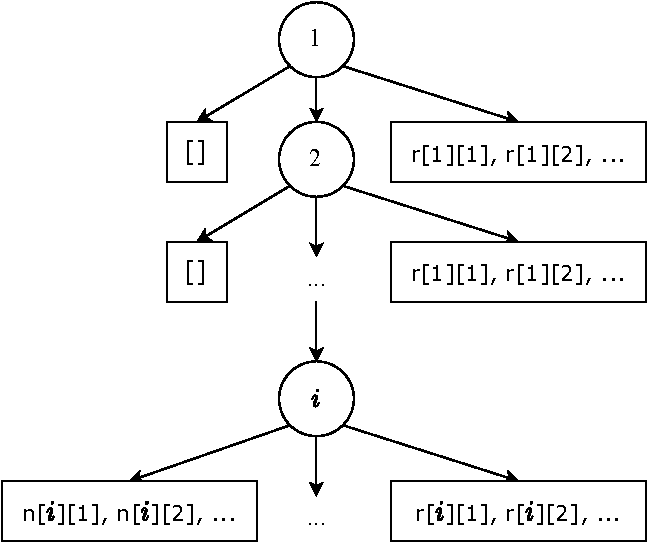
\includegraphics[scale=0.4]{img/ftr-illed-1}
  \captionof{figure}{不规则树,第$i$层子树的$f$不空}
  \label{fig:ftr-illed-form}
\end{center}

我们要从不规则的手指树中删除第一个元素。首先进行一轮自顶向下的遍历,找到一棵子树,或者它的$f$不为空,或者$f$和中间子树都为空,如图\ref{fig:ftr-illed-form}。对于前者,我们可以从$f$中提取出第一个元素(是一个节点)。对于后者,由于只有$r$不为空,我们交换$f$、$r$,转换成前一种情况。此后,我们检查从$f$中取出的节点是否为叶子。如果不是,我们需要继续提取。我们沿着父节点一直向上回溯,直到我们提取到一个叶子节点。此时我们将到达树的根节点。图\ref{fig:ftr-illed-extract}描述了这一过程。

\begin{center}
  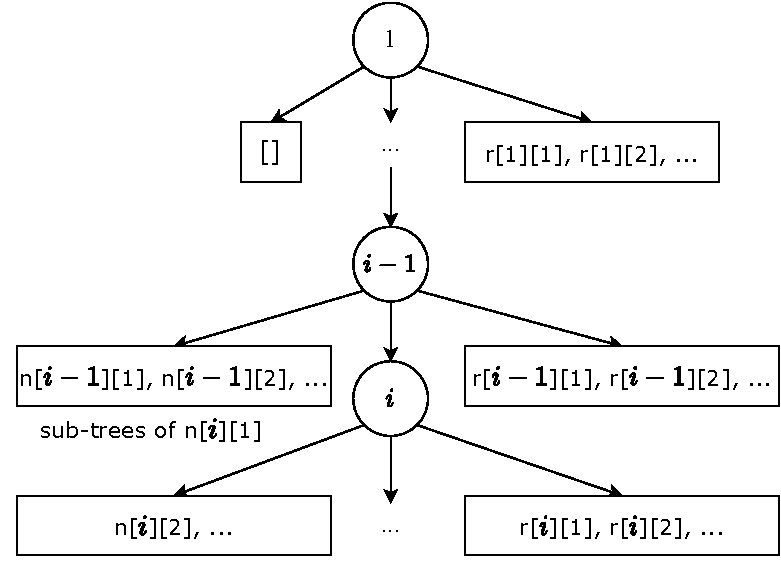
\includegraphics[scale=0.4]{img/ftr-illed-2} \\
  提取第一个元素$n[i][1]$,然后将它的子节点放到上一级树的$f$手指中。\\
  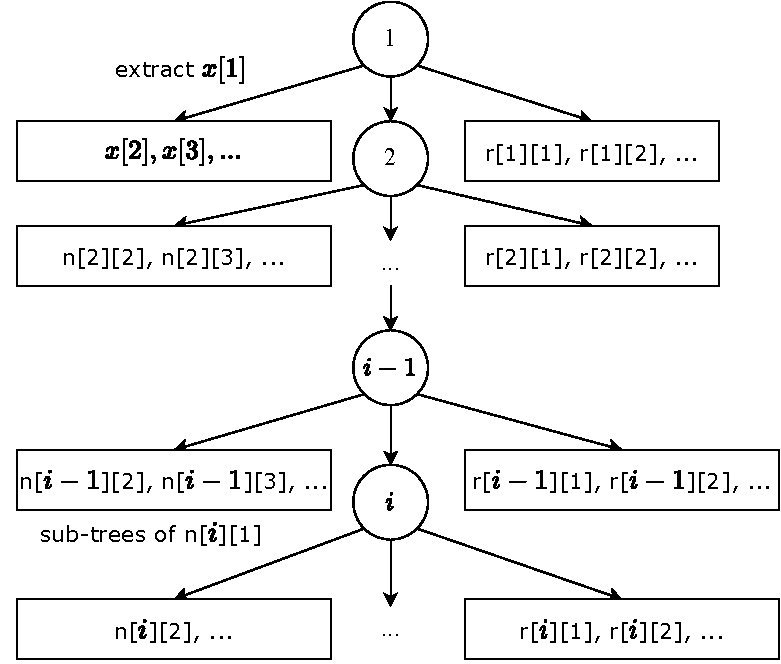
\includegraphics[scale=0.4]{img/ftr-illed-i} \\
  重复$i$次,最终提取到$x[1]$。\\
  \captionof{figure}{自底向上遍历,直到提取出一个叶子节点}
  \label{fig:ftr-illed-extract}
\end{center}

根据这一思路,下面的算法实现了列表头部的删除操作(假设树不为空)。

\begin{algorithmic}[1]
\Function{Extract}{$T$}
  \State $\perp \gets ([], T, [])$
  \While{\Call{Front}{$T$} $= [\ ]$ and \Call{Mid}{$T$} $\neq $ NIL}
    \State $T \gets$ \Call{Mid}{$T$}
  \EndWhile

  \If{\Call{Front}{$T$} $ = [\ ]$ and \Call{Rear}{$T$} $\neq [\ ]$}
    \State \textproc{Exchange} \Call{Front}{$T$} $\leftrightarrow$ \Call{Rear}{$T$}
  \EndIf

  \State $f \gets$ \Call{Front}{$T$}, $r \gets$ \Call{Rear}{$T$}
  \State $n \gets (f[1], f[2], ...)$ \Comment{$n$是2-3树}
  \Repeat
    \State \Call{Front}{$T$} $\gets [n_2, n_3, ..]$
    \State $n \gets n_1$
    \State $T \gets $ \Call{Parent}{$T$}
    \If{\Call{Mid}{$T$} becomes empty}
      \State \Call{Mid}{$T$} $\gets$ NIL
    \EndIf
  \Until{$n$ is leaf}
  \State \Return (\Call{Elem}{$n$}, \Call{Mid}{$\perp$})
\EndFunction
\end{algorithmic}

这里函数\textproc{Elem}($n$)返回叶子节点$n$中保存的唯一元素。由于不规则的树存在,需要调整从手指树中获取第一个和最后一个元素的定义。我们不再仅返回手指的第一个或者最后一个子节点。如果手指为空,而中间子树不为空,我们就沿着中间部分向下遍历,直到发现手指不为空,或者所有的节点都存储在另一侧的手指中。

\begin{algorithmic}[1]
\Function{First-Leaf}{$T$}
  \While{\Call{Front}{$T$} $ = [\ ]$ and \Call{Mid}{$T$} $\neq$ NIL}
    \State $T \gets$ \Call{Mid}{$T$}
  \EndWhile
  \If{\Call{Front}{$T$} $ = [\ ]$ and \Call{Rear}{$T$} $\neq [\ ]$}
    \State $n \gets$ \Call{Rear}{$T$}[1]
  \Else
    \State $n \gets$ \Call{Front}{$T$}[1]
  \EndIf
  \While{$n$ is NOT leaf}
    \State $n \gets n_1$
  \EndWhile
  \State \Return $n$
\EndFunction
\Statex
\Function{First}{$T$}
  \State \Return \textproc{Elem}(\Call{First-Leaf}{$T$})
\EndFunction
\end{algorithmic}

其中第二个循环中,如果节点不是叶子,就不断沿着第一个子节点遍历。获取最后一个元素与此类似.
}
\end{Answer}

\subsection{尾部操作}
\index{手指树!尾部添加}

我们可以对称地实现尾部添加、删除。

\be
\begin{array}{rcl}
append\ \nil\ a & = & (a) \\
append\ (a)\ b & = & ([a], \nil, [b]) \\
append\ (f, t, [a, b, c, d])\ e & = & (f, append\ t\ (a, b, c), [d, e]) \\
append\ (f, t, r)\ a & = & (f, t, r \doubleplus [a]) \\
\end{array}
\ee

如果$r$中的元素不超过4个,仍是合法的2-3树,我们直接把新元素添加到$r$末尾。否则,将$r$中的前三个元素取出,构造一棵新的2-3树,递归地添加到中间子树的尾部。

\index{手指树!尾部删除}

\be
\begin{array}{rcl}
remove\ (a) & = & (\nil, a) \\
remove\ ([a], \nil, [b]) & = & ((a), b) \\
remove\ (f, \nil, [a]) & = & ((init f, \nil, [last f]), a) \\
remove\ (f, t, [a]) & = & ((f, t', toList\ r), a), \text{其中}: (t', r) = remove\ t \\
remove\ (f, t, r) & = & ((f, t, init\ r), last\ r) \\
\end{array}
\ee

其中$last$获取列表的最后一个元素,$init$返回其余部分(定义见第一章)。

\subsection{连接}
\index{手指树!连接}

考虑两棵手指树都不为空的情况:$T_1 = (f_1, t_1, r_1)$、$T_2 = (f_2, t_2, r_2)$。我们用$f_1$作为连接结果中的$f$,用$r_2$作为结果中的$r$。然后将$t_1$、$r_1$、$f_2$、$t_2$合并成中间子树。由于$r_1$和$f_2$都是节点的列表,所以这等价于如下问题:

\[
merge\ t_1\ (r_1 \doubleplus f_2)\ t_2 = ?
\]

$t_1$和$t_2$也都是手指树,但它们比$T_1$和$T_2$深一级,若$T_1$中的元素类型为$a$,则$t_1$中的元素类型为$Node\ a$。我们递归地进行合并:保留$t_1$的$f$手指和$t_2$的$r$手指,然后将$t_1$和$t_2$的中间部分,$t_1$的$r$手指和$t_2$的$f$手指合并。

\be
\begin{array}{rcl}
merge\ \nil\ ts\ t_2 & = & foldr\ insert\ t_2\ ts \\
merge\ t_1\ ts\ \nil & = & foldl\ append\ t_1\ ts \\
merge\ (a)\ ts\ t_2 & = & merge\ \nil\ (a \cons ts)\ t_2 \\
merge\ t_1\ ts\ (a) & = & merge\ t_1\ (ts \doubleplus [a])\ \nil \\
merge\ (f_1, t_1, r_1)\ ts\ (f_2, t_2, r_2) & = & (f_1, merge\ t_1\ (nodes\ (r_1 \doubleplus ts \doubleplus f_2))\ t_2, r_2) \\
\end{array}
\label{eq:merge-recursion}
\ee

其中$nodes$将若干元素组织成一组2-3树。这是因为中间子树中的元素类型,比手指中的元素类深一级。

\be
\begin{array}{rcl}
nodes\ [a, b] & = & [(a, b)] \\
nodes\ [a, b, c] & = & [(a, b, c)] \\
nodes\ [a, b, c, d] & = & [(a, b), (c, d)] \\
nodes\ (a \cons b \cons c \cons ts) & = & (a, b, c) \cons nodes\ ts \\
\end{array}
\ee

这样我们可以用$merge$来定义手指树的连接:

\be
(f_1, t_1, r_1) \doubleplus (f_2, t_2, r_2) = (f_1, merge\ t_1\ (r_1 \doubleplus f_2)\ t_2, r_2)
\ee

比较这一定义和(\ref{eq:merge-recursion}),连接操作本质上就是合并操作,我们可以给出下面更加一致的定义:

\be
T_1 \doubleplus T_2 = merge\ T_1\ [\ ]\ T_2
\ee

连接的性能取决于递归的合并操作。递归的深度为两棵树中较小的一棵。由于2-3树的平衡性,手指树的高度为$O(\lg n)$其中$n$为元素的个数。合并在边界条件下的性能和插入一样(最多调用$insert$\ 8次)为分摊常数时间,最坏情况为$O(\lg m)$,其中$m$是两棵树的高度差。总体上算法的复杂度为$O(\lg n)$,其中$n$是两棵手指树中含有的元素总数。

\subsection{随机访问}
\index{手指树!随机访问}

我们的策略是把随机访问转换为树搜索。为了避免反复计算树的大小,我们给每个节点增加一个$s$变量记录其包含的元素个数:$(s, f, t, r)$。

\begin{Haskell}
data Tree a = Empty
            | Lf a
            | Tr Int [a] (Tree (Node a)) [a]
\end{Haskell}

\be
\begin{array}{rcl}
size\ \nil & = & 0 \\
size\ (x) & = & 1 \\
size\ (s, f, t, r) & = & s \\
\end{array}
\ee

我们还需要获取2-3树的大小:

\be
\begin{array}{rcl}
size\ (t_1, t_2) & = & size\ t_1 + size\ t_2 \\
size\ (t_1, t_2, t_3) & = & size\ t_1 + size\ t_2 + size\ t_3 \\
\end{array}
\ee

\index{手指树!分割}
对于节点的列表(例如深一级的手指)我们可以用$sum \circ (map\ size)$来计算大小。在插入和删除操作中,我们也需要更新树大小。增加大小信息后,给定一个位置$i$,可以通过树搜索定位到相应的节点。手指树具有递归结构:$(s, f, t, r)$,我们令这些子结构的大小为:$s_f$、$s_t$、$s_r$。如果$i \leq s_f$,则目标位于$f$中,我们接下来在$f$中查找;如果$s_f < i \leq s_f + s_t$,则目标位于$t$中,我们递归在$t$中搜索;否则目标位于$r$中。如果忽略空树,只存在一种边界情况。

\[
splitAt(i, T) = \left \{
  \begin{array}
  {r@{\quad:\quad}l}
  (\phi, x, \phi) & T = leaf(x) \\
  ... & otherwise
  \end{array}
\right .
\]

如果对叶子进行分割,则左右部分都为空,叶子中的节点就是结果。

递归的情况根据$i$的大小又分为三种子情况。设函数$splitAtL(i, L)$在位置$i$上将节点列表分割成三部分:$(A, x, B) = splitAtL(i, L)$,其中$x$为$L$中第$i$个节点,$A$是$i$前的子列表,而$B$是$i$后的子列表。

\be
splitAt(i, T) = \left \{
  \begin{array}
  {r@{\quad:\quad}l}
  (\phi, x, \phi) & T = leaf(x) \\
  (fromL(A), x, tree'(B, M, R)) & i \leq S_f\\
  (tree'(F, M_l, A), x, tree'(B, M_r, R)) & S_f < i \leq S_f + S_m \\
  (tree'(F, M, A), x, fromL(B)) & otherwise
  \end{array}
\right .
\ee

在上式第二种情况中,有$(A, x, B) = splitAtL(i, F)$;而在最后一种情况中,这一关系为:$ (A, x, B) = splitAtL(i-S_f-S_m, R)$;比较复杂的是第三种情况,其中的$M_l$、$x$、$M_r$、$A$、$B$的计算如下:

\[
\begin{array}{l}
(M_l, t, M_r) = splitAt(i-S_f, M) \\
(A, x, B) = splitAtL(i-S_f-size(M_l), unwraps(t))
\end{array}
\]

函数$splitAtL$实际上进行了线性遍历,由于列表的长度有限,且不超过2-3树的分支数目限制。因此性能仍然是常数时间$O(1)$的。记$L = \{x_1, x_2, ... \}$、$L' = \{ x_2, x_3, ...\}$。

\be
splitAtL(i, L) = \left \{
  \begin{array}
  {r@{\quad:\quad}l}
  (\phi, x_1, \phi) & i = 0 \land L = \{x_1\} \\
  (\phi, x_1, L') & i < size'(x_1) \\
  (\{x_1\} \cup A, x, B) & otherwise
  \end{array}
\right .
\ee

其中

\[
(A, x, B) = splitAtL(i-size'(x_1), L')
\]

分割的解法是典型的分而治之策略。算法的性能取决于中间部分子树的递归搜索,其他情况下都是线性时间。递归的深度和树的高度$h$成比例,因此算法的性能为$O(h)$。由于树是平衡的(使用2-3树,且所有的插入、删除等操作都维持树的平衡),所以$h = O(\lg n)$,其中$n$是树中存储的元素数目。分割算法的整体性能为$O(\lg n)$。

下面的Haskell例子程序给出了$splitAtL$算法的实现。

\lstset{language=Haskell}
\begin{lstlisting}[style=Haskell]
splitNodesAt 0 [x] = ([], x, [])
splitNodesAt i (x:xs) | i < size x = ([], x, xs)
                      | otherwise = let (xs', y, ys) = splitNodesAt (i-size x) xs
                                    in (x:xs', y, ys)
\end{lstlisting}

由于Haskell的标准库中已经定义了同样名字的\texttt{splitAt}函数,为了避免冲突,我们将名称改为\texttt{splitAt'}。

\begin{lstlisting}[style=Haskell]
splitAt' _ (Lf x) = (Empty, x, Empty)
splitAt' i (Tr _ f m r)
    | i < szf = let (xs, y, ys) = splitNodesAt i f
                in ((foldr cons' Empty xs), y, tree ys m r)
    | i < szf + szm = let (m1, t, m2) = splitAt' (i-szf) m
                          (xs, y, ys) = splitNodesAt (i-szf - sizeT m1) (unwraps t)
                      in (tree f m1 xs, y, tree ys m2 r)
    | otherwise = let (xs, y, ys) = splitNodesAt (i-szf -szm) r
                  in (tree f m xs, y, foldr cons' Empty ys)
    where
      szf = sizeL f
      szm = sizeT m
\end{lstlisting}

\subsubsection{随机访问}
\index{手指树!随机访问}

使用分割算法,我们可以很容易地实现性能为$O(\lg n)$的随机访问。令函数$mid(x)$返回一个三元组的第2个部分,$left(x)$和$right(x)$分别返回第1和第3部分。

\be
getAt(S, i) = unwrap(mid(splitAt(i, S)))
\ee

我们首先在位置$i$将序列分成3部分,然后取出返回的节点,并得到其中的元素。如果希望修改序列中的第$i$个元素,我们首先用$i$来分割,然后将中间部分替换成要修改的值,最后再使用连接操作将这三部分合并起来。

\be
setAt(S, i, x) = concat(L, insertT(x, R))
\ee

其中
\[
(L, y, R) = splitAt(i, S)
\]

更进一步,我们还可以实现$removeAt(S, i)$算法,从一个序列$S$中删除第$i$个元素。我们首先用位置$i$分割,将节点中的元素返回,然后将左侧和右侧部分连接成一棵新手指树。

\be
removeAt(S, i) = (unwrap(y), concat(L, R))
\ee

下面的Haskell例子程序实现了这些操作。

\lstset{language=Haskell}
\begin{lstlisting}[style=Haskell]
getAt t i = unwrap x where (_, x, _) = splitAt' i t
setAt t i x = let (l, _, r) = splitAt' i t in concat' l (cons x r)
removeAt t i = let (l, x, r) = splitAt' i t in (unwrap x, concat' l r)
\end{lstlisting}

\subsubsection{命令式随机访问}
\index{手指树!命令式随机访问}

在命令式环境中,我们可以直接修改树中的值,因此可以不用分割而直接实现\textproc{Get-At}($T, i$)和\textproc{Set-At}($T, i, x$)算法。我们先实现一个通用算法,可以在给定位置执行指定的操作。下面的算法接受三个参数,一棵手指树$T$,一个从0开始的位置索引$i$,以及一个函数$f$,用以对位置$i$上的元素实施操作。

\begin{algorithmic}
\Function{Apply-At}{$T, i, f$}
  \While{\Call{Size}{$T$} $> 1$}
    \State $S_f \gets $ \textproc{Size-Nodes}(\Call{Front}{$T$})
    \State $S_m \gets $ \textproc{Size-Tr}(\Call{Mid}{$T$})
    \If{$i < S_f$}
      \State \Return \textproc{Lookup-Nodes}(\Call{Front}{$T$}, $i$, $f$)
    \ElsIf{$i < S_f + S_m$}
      \State $T \gets$ \Call{Mid}{$T$}
      \State $i \gets i - S_f$
    \Else
      \State \Return \textproc{Lookup-Nodes}(\Call{Rear}{$T$}, $i - S_f - S_m$, $f$)
    \EndIf
  \EndWhile
  \State $n \gets$ \Call{First-Lf}{$T$}
  \State $x \gets$ \Call{Elem}{$n$}
  \State \Call{Elem}{$n$} $\gets f(x)$
  \State \Return $x$
\EndFunction
\end{algorithmic}

算法本质上是一个分而治之的树搜索。它不断检查当前的树直到树的size为1(可以通过是否是叶子来进行判断么?请考虑后面练习中的不规则树)。每次循环,我们都检查$i$、front手指的size,和中间部分子树的size之间的关系。

如果索引$i$小于front手指的size,则节点在front手指中。算法就调用一个子过程在front手指中查找;如果索引不比front手指的size小,但是比加上中间部分子树的size的结果小,则节点在中间部分,算法就从$i$中减去front手指的size,然后继续遍历中间部分的子树;否则,说明节点在rear手指中,算法调用子过程在其中查找。

循环结束后,我们得到一个节点(可能是一个复合节点),待查找的元素存储于这一节点的第一个叶子中。我们可以将它取出,然后对其执行函数$f$,并将结果存回树中。

算法返回执行$f$前的元素作为最终结果。

接下来我们需要实现算法\textproc{Lookup-Nodes}($L$, $i$, $f$)。它接受三个参数:一个节点列表,一个位置索引,和一个待执行的函数。我们可以逐一检查列表中的每个节点,如果节点为叶子,并且位置索引为0,我们恰巧到达了指定位置。我们在这个叶子的元素上执行函数,并将此前的元素值返回;否则,我们需要比较节点的size和位置索引,以决定是否仅需在这个节点中搜索。

\begin{algorithmic}
\Function{Lookup-Nodes}{$L, i, f$}
  \Loop
    \For{$\forall n \in L$}
      \If{$n$ is leaf $\land i = 0$}
        \State $x \gets $ \Call{Elem}{$n$}
        \State \Call{Elem}{$n$} $\gets f(x)$
        \State \Return $x$
      \EndIf
      \If{$i < $ \Call{Size}{$n$}}
        \State $L \gets $ \Call{Children}{$n$}
        \State break
      \EndIf
      \State $i \gets i - $ \Call{Size}{$n$}
    \EndFor
  \EndLoop
\EndFunction
\end{algorithmic}

下面的Python例子程序实现了这一算法。

\lstset{language=Python}
\begin{lstlisting}
def applyAt(t, i, f):
    while t.size > 1:
        szf = sizeNs(t.front)
        szm = sizeT(t.mid)
        if i < szf:
            return lookupNs(t.front, i, f)
        elif i < szf + szm:
            t = t.mid
            i = i - szf
        else:
            return lookupNs(t.rear, i - szf - szm, f)
    n = first_leaf(t)
    x = elem(n)
    n.children[0] = f(x)
    return x

def lookupNs(ns, i, f):
    while True:
        for n in ns:
            if n.leaf and i == 0:
                x = elem(n)
                n.children[0] = f(x)
                return x
            if i < n.size:
                ns = n.children
                break
            i = i - n.size
\end{lstlisting}

通过将某些特殊函数传入这一通用算法,我们就可以实现\textproc{Get-At}和\textproc{Set-At}操作。

\begin{algorithmic}
\Function{Get-At}{$T, i$}
  \State \Return \Call{Apply-At}{$T, i, \lambda_x . x$}
\EndFunction
\Statex
\Function{Set-At}{$T, i, x$}
  \State \Return \Call{Apply-At}{$T, i, \lambda_y . x$}
\EndFunction
\end{algorithmic}

我们传入$id$函数来获取指定位置的元素,它并不改变元素的值;通过传入常数函数,我们可以实现设置,它忽略元素以前的值,而将传入的值作为新结果。

\subsubsection{命令式分割}
\index{手指树!命令式分割}

在命令式环境下,仅仅实现\textproc{Apply-At}算法还不够,我们还需要能删除指定位置的元素。

此前我们介绍的所有命令式手指树算法都只执行一轮自顶向下的操作。由于不需要自底向上进行回溯。所以,父节点到目前为止还没有派上用场。

使用父节点可以容易地实现分割操作。我们首先沿着中间部分的子树执行一轮自顶向下的遍历,直到分割位置落入front手指或者rear手指。此后,我们沿着父节点分别向上回溯两棵分割树以填入相应的内容。

\begin{algorithmic}
\Function{Split-At}{$T, i$}
  \State $T_1 \gets$ \textproc{Tree}()
  \State $T_2 \gets$ \textproc{Tree}()
  \While{$S_f \leq i < S_f + S_m$} \Comment{自顶向下遍历}
    \State $T'_1 \gets$ \textproc{Tree}()
    \State $T'_2 \gets$ \textproc{Tree}()
    \State \Call{Front}{$T'_1$} $\gets$ \Call{Front}{$T$}
    \State \Call{Rear}{$T'_2$} $\gets$ \Call{Rear}{$T$}
    \State \Call{Connect-Mid}{$T_1, T'_1$}
    \State \Call{Connect-Mid}{$T_2, T'_2$}
    \State $T_1 \gets T'_1$
    \State $T_2 \gets T'_2$
    \State $i \gets i - S_f$
    \State $T \gets$ \Call{Mid}{$T$}
  \EndWhile

  \If{$i < S_f$}
    \State $(X, n, Y) \gets$ \textproc{Split-Nodes}(\Call{Front}{$T$}, $i$)
    \State $T'_1 \gets$ \Call{From-Nodes}{$X$}
    \State $T'_2 \gets T$
    \State \Call{Size}{$T'_2$} $\gets$ \Call{Size}{$T$} - \Call{Size-Nodes}{$X$} - \Call{Size}{$n$}
    \State \Call{Front}{$T'_2$} $\gets Y$
  \ElsIf{$S_f + S_m \leq i$}
    \State $(X, n, Y) \gets$ \textproc{Split-Nodes}(\Call{Rear}{$T$}, $i - S_f - S_m$)
    \State $T'_2 \gets$ \Call{From-Nodes}{$Y$}
    \State $T'_1 \gets T$
    \State \Call{Size}{$T'_1$} $\gets$ \Call{Size}{$T$} - \Call{Size-Nodes}{$Y$} - \Call{Size}{$n$}
    \State \Call{Rear}{$T'_1$} $\gets X$
  \EndIf
  \State \Call{Connect-Mid}{$T_1, T'_1$}
  \State \Call{Connect-Mid}{$T_2, T'_2$}

  \State $i \gets i -$ \Call{Size-Tr}{$T'_1$}
  \While{$n$ is NOT leaf} \Comment{自底向上回溯}
    \State $(X, n, Y) \gets$ \textproc{Split-Nodes}(\Call{Children}{$n$}, $i$)
    \State $i \gets i -$ \Call{Size-Nodes}{$X$}
    \State \Call{Rear}{$T_1$} $\gets X$
    \State \Call{Front}{$T_2$} $\gets Y$
    \State \Call{Size}{$T_1$} $\gets$ \Call{Sum-Sizes}{$T_1$}
    \State \Call{Size}{$T_2$} $\gets$ \Call{Sum-Sizes}{$T_2$}
    \State $T_1 \gets$ \Call{Parent}{$T_1$}
    \State $T_2 \gets$ \Call{Parent}{$T_2$}
  \EndWhile

  \State \Return (\Call{Flat}{$T_1$}, \Call{Elem}{$n$}, \Call{Flat}{$T_2$})
\EndFunction
\end{algorithmic}

算法首先创建两棵树$T_1$和$T_2$来保存分割的结果。它们的含义都是“ground”树,为结果树的父节点。第一轮遍历是自顶向下的。令$S_f$和$S_m$分别是front手指和中间部分子树的size。如果待分割的位置落在中间部分的子树中,我们就使用$T$的front手指作为新建的$T'_1$的front手指;并且复用$T$的rear手指作为$T'_2$的rear手指。此时,我们还不能设置$T'_1$和$T'_2$的其他部分,它们仍然为空,我们将在此后填入必要的信息。然后,我们将$T_1$和$T'_1$连接起来,使得后者成为前者的中间部分子树;同样我们把$T_2$和$T'_2$连接起来。最后,我们从分割位置中减去front手指的size,然后继续沿着中间部分的子树遍历。

第一轮遍历结束后,我们到达一个位置,分割要么发生在front手指,要么发生在rear手指。在手指中分割会产生一个三元组,第一部分和第三部分为分割位置前后的子列表,第二部分是包含指定位置元素的节点。两个手指本质上都是2-3树,它们都最多含有3个节点,节点分割算法可以通过线性查找来完成。

\begin{algorithmic}
\Function{Split-Nodes}{$L, i$}
  \For{$j \in [1, $ \Call{Length}{$L$} $]$}
    \If{$i <$ \Call{Size}{$L[j]$}}
      \State \Return ($L[1...j-1]$, $L[j]$, $L[j+1...$ \Call{Length}{$L$} $]$)
    \EndIf
    \State $i \gets i -$ \Call{Size}{$L[j]$}
  \EndFor
\EndFunction
\end{algorithmic}

接下来,我们从三元组创建两个新的树$T'_1$和$T'_2$,然后将它们连接起来作为$T_1$和$T_2$的最终中间子树。

此后,我们需要执行自底向上的回溯。沿着结果树填入所有尚为空的部分。

我们对三元组的第二部分,也就是节点,执行循环。直到它变为一个叶子。每次循环我们不断将节点的子树用更新的位置$i$进行分割。分割结果的第一部分子列表用于填入$T_1$作为rear手指;分割结果的另一部分子列表用于填入$T_2$作为front手指。此后,由于手指树的三个部分:front手指、中间部分子树、和rear手指都完整填入了,我们就可以计算出三部分的size并相加,将结果作为树的size。

\begin{algorithmic}
\Function{Sum-Sizes}{$T$}
  \State \Return \textproc{Size-Nodes}(\Call{Front}{$T$}) + \textproc{Size-Tr}(\Call{Mid}{$T$}) + \textproc{Size-Nodes}(\Call{Rear}{$T$})
\EndFunction
\end{algorithmic}

接着,迭代继续沿着$T_1$和$T_2$的父节点进行。最后需要实现的算法是\textproc{From-Nodes}($L$)。它从一组节点创建一棵手指树。我们可以逐一将节点插入到一棵空树中实现它。我们把它作为练习留给读者。

下面的Python例子程序实现了分割算法。

\lstset{language=Python}
\begin{lstlisting}
def splitAt(t, i):
    (t1, t2) = (Tree(), Tree())
    while szf(t) <= i and i < szf(t) + szm(t):
        fst = Tree(0, t.front, None, [])
        snd = Tree(0, [], None, t.rear)
        t1.set_mid(fst)
        t2.set_mid(snd)
        (t1, t2) = (fst, snd)
        i = i - szf(t)
        t = t.mid

    if i < szf(t):
        (xs, n, ys) = splitNs(t.front, i)
        sz = t.size - sizeNs(xs) - n.size
        (fst, snd) = (fromNodes(xs), Tree(sz, ys, t.mid, t.rear))
    elif szf(t) + szm(t) <= i:
        (xs, n, ys) = splitNs(t.rear, i - szf(t) - szm(t))
        sz = t.size - sizeNs(ys) - n.size
        (fst, snd) = (Tree(sz, t.front, t.mid, xs), fromNodes(ys))
    t1.set_mid(fst)
    t2.set_mid(snd)

    i = i - sizeT(fst)
    while not n.leaf:
        (xs, n, ys) = splitNs(n.children, i)
        i = i - sizeNs(xs)
        (t1.rear, t2.front) = (xs, ys)
        t1.size = sizeNs(t1.front) + sizeT(t1.mid) + sizeNs(t1.rear)
        t2.size = sizeNs(t2.front) + sizeT(t2.mid) + sizeNs(t2.rear)
        (t1, t2) = (t1.parent, t2.parent)

    return (flat(t1), elem(n), flat(t2))
\end{lstlisting}

下面的例子程序将一个节点的列表在指定位置分割开。

\begin{lstlisting}
def splitNs(ns, i):
    for j in range(len(ns)):
        if i < ns[j].size:
            return (ns[:j], ns[j], ns[j+1:])
        i = i - ns[j].size
\end{lstlisting}

使用分割算法,就可以方便地实现删除操作了。我们首先执行分割,然后将结果中的两棵树连接成一棵,并将指定位置的元素返回。

\begin{algorithmic}
\Function{Remove-At}{$T, i$}
  \State $(T_1, x, T_2) \gets$ \Call{Split-At}{$T, i$}
  \State \Return $(x, $ \Call{Concat}{$T_1, T_2$} $)$
\EndFunction
\end{algorithmic}

\begin{Exercise}
\begin{enumerate}
\item 另外一种实现$insertT'$的方法是直接将size加1,这样我们就无需使用$tree'$函数。请实现这一方法。

\item 参考$insertT'$的实现,完成下面的算法(分别给出函数式和命令式实现):$extractT'$、$appendT'$、$removeT'$、和$concat'$。而$head$、$tail$、$init$、和$last$保持不变。

\item 在命令式算法\textproc{Apply-At}中,我们检查当前树的size是否比1大。为什么不能检查当前的节点是否为叶子?两种方法有何区别?

\item 选择一门命令式语言,实现\textproc{From-Nodes}($L$)算法。可以使用循环或者从右侧fold。
\end{enumerate}
\end{Exercise}

% ================================================================
%                 Short summary
% ================================================================
\section{小结}

虽然我们未能给出一个在常数时间$O(1)$随机访问的纯函数式列表,但是最终的手指树数据结构实现了一个总体表现良好的序列。在头部和尾部的操作的性能为分摊时间$O(1)$,可以在对数时间内连接两个序列,或者在任何位置将序列分割。命令式环境中的纯数组和函数式环境中的列表都无法同时满足这些要求。某些函数式编程环境的标准库也提供了这样的序列实现\cite{hackage-ftr}。

如本章的题目所说,我们介绍了函数式环境和命令式环境中的最后一个初等数据结构。我们可以使用它们来解决一些典型问题了。

\index{MTF}
例如,当实现一个MTF(move-to-front)的编码算法时\cite{mtf-wiki},就可以使用本章介绍的序列。

\[
mtf(S, i) = \{x\} \cup S' \\
\]

其中$(x, S') = removeAt(S, i)$。

接下来的章节中,我们将介绍一些典型的分而治之的排序算法,包括快速排序,归并排序以及它们的变形;然后我们介绍一些初等搜索算法,包括一些字符串匹配算法。
% This is planned in the 2nd edition
%finally,
%we'll give a real-world example of algorithms, BWT (Burrows-Wheeler transform) compressor,
%which is one of the best compression tool in the world.

% ================================================================
%                 Appendix
% ================================================================

\section{附录:例子程序}

随机访问列表(森林):

\lstset{frame = single}
\begin{Haskell}
data Tree a = Leaf a
            | Node Int (Tree a) (Tree a)

type BRAList a = [Tree a]

size (Leaf _) = 1
size (Node sz _ _) = sz

link t1 t2 = Node (size t1 + size t2) t1 t2

insert x = insertTree (Leaf x) where
    insertTree t [] = [t]
    insertTree t (t':ts) = if size t < size t' then  t:t':ts
                           else insertTree (link t t') ts

extract ((Leaf x):ts) = (x, ts)
extract ((Node _ t1 t2):ts) = extract (t1:t2:ts)

head' = fst . extract
tail' = snd . extract

getAt i (t:ts) | i < size t = lookupTree i t
               | otherwise = getAt (i - size t) ts
  where
    lookupTree 0 (Leaf x) = x
    lookupTree i (Node sz t1 t2)
        | i < sz `div` 2 = lookupTree i t1
        | otherwise = lookupTree (i - sz `div` 2) t2
\end{Haskell}

随机访问森林的数值表示:
\begin{Haskell}
data Digit a = Zero | One (Tree a)

type RAList a = [Digit a]

insert x = add (Leaf x) where
  add t [] = [One t]
  add t (Zero:ts) = One t : ts
  add t (One t' :ts) = Zero : add (link t t') ts

minus [One t] = (t, [])
minus (One t:ts) = (t, Zero:ts)
minus (Zero:ts) = (t1, One t2:ts') where
    (Node _ t1 t2, ts') = minus ts

head' ts = x where (Leaf x, _) = minus ts
tail' = snd . minus
\end{Haskell}

双数组序列:

\begin{lstlisting}[language = Bourbaki]
Data Seq<K> {
    [K] front = [], rear = []
}

Int length(S<K> s) = length(s.front) + length(s.rear)

void insert(K x, Seq<K> s) = append(x, s.front)

void append(K x, Seq<K> s) = append(x, s.rear)

K get(Int i, Seq<K> s) {
    Int n = length(s.front)
    return if i < n then s.front[n - i - 1] else s.rear[i - n]
}
\end{lstlisting}

可连接列表:

\begin{Haskell}
data CList a = Empty | CList a (Queue (CList a))

wrap x = CList x emptyQ

x ++ Empty = x
Empty ++ y = y
(CList x q) ++ y = CList x (push q y)

fold f z q | isEmpty q = z
           | otherwise = (top q) `f` fold f z (pop q)

concat = fold (++) Empty

insert x xs = (wrap x) ++ xs
append xs x = xs ++ wrap x

head (CList x _) = x
tail (CList _ q) = concat q
\end{Haskell}

\ifx\wholebook\relax \else
\section{参考答案}
\shipoutAnswer

\begin{thebibliography}{99}

\bibitem{okasaki-book}
Chris Okasaki. ``Purely Functional Data Structures''. Cambridge university press, (July 1, 1999), ISBN-13: 978-0521663502

\bibitem{okasaki-ralist}
Chris Okasaki. ``Purely Functional Random-Access Lists''. Functional Programming Languages and Computer Architecture, June 1995, pages 86-95.

\bibitem{CLRS}
Thomas H. Cormen, Charles E. Leiserson, Ronald L. Rivest and Clifford Stein. ``Introduction to Algorithms, Second Edition''. The MIT Press, 2001. ISBN: 0262032937.(《算法导论》中文版)

\bibitem{learn-haskell}
Miran Lipovaca. ``Learn You a Haskell for Great Good! A Beginner's Guide''. No Starch Press; 1 edition April 2011, 400 pp. ISBN: 978-1-59327-283-8

\bibitem{finger-tree-2006}
Ralf Hinze and Ross Paterson. ``Finger Trees: A Simple General-purpose Data Structure,'' in Journal of Functional Programming 16:2 (2006), pages 197-217. \url{http://www.soi.city.ac.uk/~ross/papers/FingerTree.html}

\bibitem{finger-tree-1977}
Guibas, L. J., McCreight, E. M., Plass, M. F., Roberts, J. R. (1977), "A new representation for linear lists". Conference Record of the Ninth Annual ACM Symposium on Theory of Computing, pp. 49-60.

\bibitem{hackage-ftr}
Generic finger-tree structure. \url{http://hackage.haskell.org/packages/archive/fingertree/0.0/doc/html/Data-FingerTree.html}

\bibitem{mtf-wiki}
Wikipedia. Move-to-front transform. \url{https://en.wikipedia.org/wiki/Move-to-front_transform}

\end{thebibliography}

\expandafter\enddocument
\fi
